\documentclass[a4paper,fleqn,12pt]{article}
\usepackage{mathtools}
%\usepackage{amsthm}
\usepackage{amsmath}
%\usepackage{nccmath}
\usepackage{amssymb}
%\usepackage{amsfonts}
\usepackage{physics}
%\usepackage{dsfont}
%\usepackage{mathrsfs}
%\usepackage{slashed}    % Feynman slash notation, requires LuaLaTeX
%\usepackage[compat=1.1.0]{tikz-feynman}   % Feynman diagrams

%\usepackage{titling}
\usepackage{indentfirst}
%\usepackage[titletoc,title]{appendix}
%\renewcommand\appendixname{Apêndice}

\usepackage{bm}
%\usepackage{xcolor}
%\usepackage[dvipsnames]{xcolor}
\usepackage{cancel}

%\usepackage{xurl}
\usepackage{hyperref}
\usepackage{cite}

\usepackage{float}
\usepackage{graphicx}
\usepackage{tikz}
\usepackage{caption}
\usepackage{subcaption}

%%%%%%%%%%%%%%%%%%%%%%%%%%%%%%%%%%%%%%%%%%%%%%%%%%%

\newcommand{\eps}{\epsilon}
\newcommand{\vphi}{\varphi}
\newcommand{\cte}{\text{cte}}

\newcommand{\N}{\mathbb{N}}
\newcommand{\Z}{\mathbb{Z}}
\newcommand{\Q}{\mathbb{Q}}
\newcommand{\R}{\mathbb{R}}
\newcommand{\C}{\mathbb{C}}
\renewcommand{\P}{\mathbb{P}}
\renewcommand{\H}{\s{H}}

\newcommand{\0}{\vb{0}}
\newcommand{\1}{\mathds{1}}
\newcommand{\E}{\vb{E}}
\newcommand{\B}{\vb{B}}
\renewcommand{\v}{\vb{v}}
\renewcommand{\r}{\vb{r}}
\newcommand{\p}{\vb{p}}
\newcommand{\q}{\vb{q}}
\newcommand{\F}{\vb{F}}
\newcommand{\dtcp}{\delta_{\text{CP}}}

\newcommand{\s}[1]{\mathcal{#1}}
\renewcommand{\sl}[1]{\slashed{#1}}
\newcommand{\prodint}[2]{\left\langle #1 , #2 \right\rangle}
\newcommand{\cc}[1]{\overline{#1}}
\newcommand{\Eval}[3]{\eval{\left( #1 \right)}_{#2}^{#3}}

\newcommand{\unit}[1]{\; \mathrm{#1}}

\newcommand{\n}{\medskip}
\newcommand{\e}{\quad \mathrm{e} \quad}
\newcommand{\ou}{\quad \mathrm{ou} \quad}
\newcommand{\virg}{\, , \;}
\newcommand{\ptodo}{\forall \,}
\newcommand{\existe}{\exists \,}
\renewcommand{\implies}{\; \Rightarrow \;}
%\newcommand{\eqname}[1]{\tag*{#1}} % Tag equation with name

% MACROS
\newcommand{\dcp}{\delta_{\text{CP}}}


\title{\Huge{\textbf{KamLAND}}}
\author{Mateus Marques}

\begin{document}

\maketitle

\section{LEMBRETE}

Uma linha do ano de 2022 para o reator \texttt{hanbit-6} (Yonggwang) tem dados faltantes. Estimei o dado de \texttt{LF-An} com base no \texttt{TimeOnLine} e \texttt{RefUnitPow}, supondo que \texttt{LF-An} seja proporcional ao \texttt{TimeOnLine}, e que o funcionamento é o mesmo para um ano de mesma \texttt{RefUnitPow}.

\section{``Evidence of Spectral Distortion''}

\subsection{Fission rates}

``\textit{KamLAND is surrounded by 53 Japanese power reactor units.
The reactor operation data, including thermal
power generation, fuel burn up, exchange and enrichment
records, are provided by all Japanese power reactors and
are used to calculate fission rates of each isotope.
The averaged relative fission yields for the run period were}

$^{235}\text{U} : ^{238}\text{U} : ^{239}\text{Pu} : ^{241}\text{Pu} = 0.563: 0.079 : 0.301: 0.057$.

\textit{The expected $\cc{\nu}_e$ flux is calculated using fission rates and $\cc{\nu}_e$ spectra; the spectra are from Ref. [3].''}

\n\n

Se olharmos a referência [3] citada acima, vemos:

\begin{itemize}
\item $^{235}\text{U}$ : K. Schreckenbach et al., Phys. Lett. B 160, 325 (1985); \texttt{schrecken1985}.

\item $^{239,241}\text{Pu}$ : A. A. Hahn et al., Phys. Lett. B 218, 365 (1989); \texttt{hahn1989}.

\item $^{238}\text{U}$ : P. Vogel et al., Phys. Rev. C 24, 1543 (1981); \texttt{vogel1981}.
\end{itemize}

Esses três artigos estão na pasta \texttt{ccc}.

\subsection{General}

Essa análise é entre 9 de Maio, 2002 e 11 de Janeiro, 2004.

\section{DetwillerThesis}

The remaining ingredients in the signal calculation (see Equation 2.3) are the resolu-
tion function $R(E_p, E_{\cc{\nu}_e}')$ described by Equations 2.2 and 4.10, the number of target
protons $n_p$ calculated in Section 5.6, the cross-section $\sigma_{E_{\cc{\nu}_e}}$ taken from [52]


[52] P. Vogel and J.F. Beacom, Phys. Rev. D 60, 053003 (1999); radiative correction
from A. Kurylov, et al., Phys. Rev. C 67, 035502 (2003).

Temos $E = E_p$ e $E' = E_{\cc{\nu}_e}'$.

$$
\frac{\dd[2]{N_{\cc{\nu}_e}}}{\dd{E}\dd{t}} =
\int_0^\infty \dd{E'} \, R(E, E') \, n_p \, \sigma(E') \eps(E')
\sum_{i}^{\text{reactors}} \frac{I_i(E', t)}{4\pi L_i^2}
P_{\cc{\nu}_e \to \cc{\nu}_e}(E', L_i).
$$

$$
I_i(E) = \sum^{\text{isotopes}}_{k} f_{i,k}(t)
\dv{N_{\cc{\nu}_e, k} (E)}{E}.
$$

$$
\phi_{\cc{\nu}_e}(t) =
\sum_{i}^{\text{reactors}} \phi_{\cc{\nu}_e, i}(t) =
\sum_{i}^{\text{reactors}} \frac{1}{4\pi L_i^2}
\int_0^\infty I_i(E_{\cc{\nu}_e}', t) \dd{E_{\cc{\nu}_e}'}.
$$

Definindo então
$$
\Phi_{\cc{\nu}_e, i} = \int_{\text{start}}^{\text{end}} \phi_{\cc{\nu}_e, i}(t) \dd{t},
$$
temos
$$
something.
$$

\section{Tohoku website}

\begin{figure}[H]
\centering
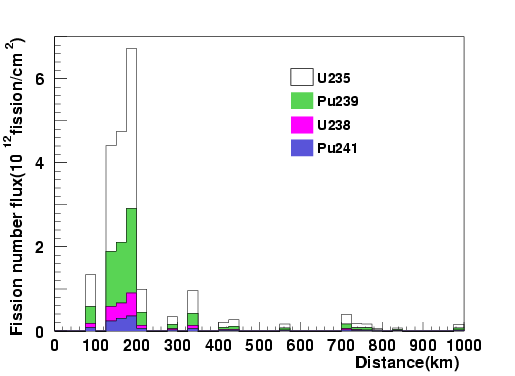
\includegraphics[width=0.7\textwidth]{fig/calc_by_run_time_distance_graph.png}
\caption{Integrated fission flux at the Kamioka site for the four main nuclei that have fission products contributing to the anti-neutrino flux from reactors up to a distance of 1000km from the experimental site}
\label{fig:calc_by_run_time_distance_graph}
\end{figure}

The four main fission nuclei are U-235, U-238, Pu-239 and Pu-241 and their fission fluxes, integrated over the total detector livetime, are provided in the data file \texttt{fission\_flux\_distance.dat}.





\end{document}
